\chapter*{Proposition 30}



\begin{figure*}[ht]
    \begin{center}
    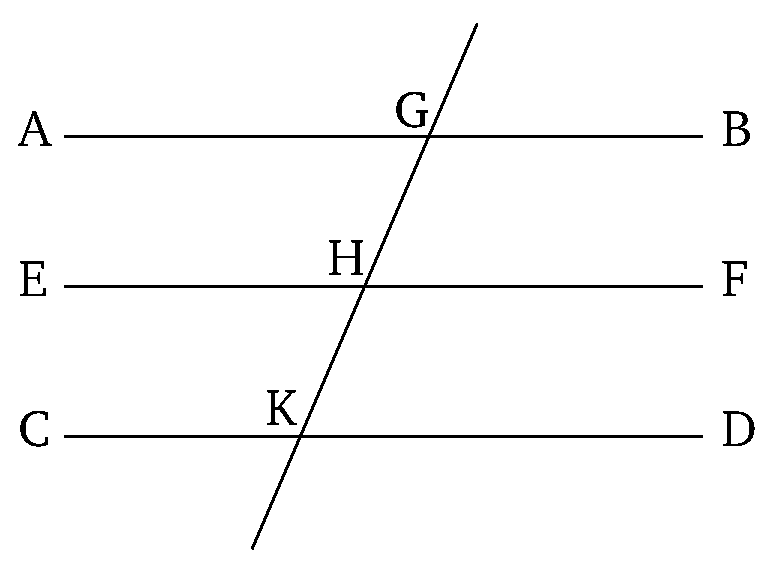
\includegraphics[width=0.5\linewidth]{figures/fig30e.eps}
    \label{fig:prop_30}
    \end{center}
\end{figure*}

(Straight-lines) parallel to the same straight-line are also parallel
to one another.

Let each of the (straight-lines) $AB$ and $CD$ be parallel to $EF$. I say that
$AB$ is also parallel to $CD$.

For let the straight-line $GK$ fall across  ($AB$, $CD$, and $EF$).

And since the straight-line $GK$ has fallen across the parallel straight-lines $AB$ and $EF$, (angle) $AGK$
(is) thus equal to $GHF$ [Prop.~1.29]. Again, since the straight-line $GK$ has fallen across the parallel
straight-lines $EF$ and $CD$, (angle) $GHF$ is equal to $GKD$ [Prop.~1.29].
But $AGK$ was also shown (to be) equal to $GHF$. Thus, $AGK$ is also equal to 
$GKD$. And they are alternate (angles). Thus, $AB$ is parallel to $CD$ [Prop.~1.27].

\mbox{[}Thus, (straight-lines) parallel to the same straight-line are also parallel
to one another.] (Which is) the very thing it was required to show.


\section*{Commentary}

\begin{proposition}\label{proposition_30}\lean{Elements.Book1.proposition_30}\leanok
    If
\end{proposition}
\begin{proof}
    \uses{proposition_27,proposition_29}\leanok
\end{proof}
